\documentclass[11pt,a4paper]{article}

\usepackage[T1]{fontenc}
\usepackage[utf8]{inputenc}
\usepackage{lmodern}
\usepackage{microtype}
\usepackage[margin=2.5cm]{geometry}
\usepackage{amsmath,amssymb}
\usepackage{booktabs}
\usepackage{array}
\usepackage{xcolor}
\usepackage{tikz}
\usetikzlibrary{arrows.meta,positioning}
\usepackage{float}
\usepackage{algorithm}
\usepackage{algpseudocode}
\usepackage{enumitem}
\usepackage{titlesec}
\usepackage[hidelinks]{hyperref}

\definecolor{accent}{HTML}{1F4E79}
\definecolor{boxfill}{HTML}{EAF1F8}

\titleformat{\section}{\Large\bfseries\color{accent}}{\thesection}{0.6em}{}
\titleformat{\subsection}{\normalsize\bfseries}{\thesubsection}{0.6em}{}
\setlist{itemsep=2pt,topsep=4pt}
\setlength{\parindent}{0pt}
\setlength{\parskip}{6pt}

\newcommand{\E}{\mathbb{E}}
\newcommand{\Normal}{\mathcal{N}}

\begin{document}
\begin{center}
{\LARGE\bfseries\color{accent} PITWALL}\\[6pt]
{\large Algorithms and Mathematics of a 1v1 F1\\ Opponent-Prediction and Counter-Strategy Engine}\\[6pt]
{\small November 2026}
\end{center}
\vspace{-0.5em}

\begin{abstract}
\noindent PITWALL estimates tyre degradation from public lap times, predicts when an
opponent will pit, and simulates our options to the end of the race to recommend one.
It chains five simple, explainable models rather than one large one. This document
sets out the mathematics of each model, the assumptions behind it, and how the
system was evaluated, including where it falls short. A live terminal runs the same models
during a race and is scored against real results from unseen 2025 and 2026 races. Meta's
Muse Spark then answers an engineer's questions about each call, using only the system's numbers.
It explains the call and cannot change it.
\end{abstract}

\section{System overview}

The pipeline runs once per lap and may use only laps that have already been completed.

\begin{figure}[H]
\centering
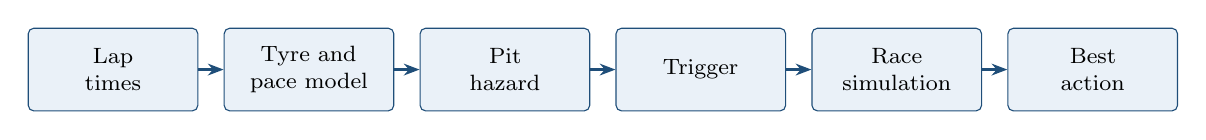
\begin{tikzpicture}[
  node distance=0.32cm,
  box/.style={draw=accent,fill=boxfill,rounded corners=2pt,align=center,
              minimum height=1.05cm,text width=1.92cm,font=\footnotesize},
  arr/.style={-{Stealth[length=2mm]},accent,thick}]
\node[box] (a) {Lap\\times};
\node[box,right=of a] (b) {Tyre and\\pace model};
\node[box,right=of b] (c) {Pit\\hazard};
\node[box,right=of c] (d) {Trigger};
\node[box,right=of d] (e) {Race\\simulation};
\node[box,right=of e] (f) {Best\\action};
\foreach \x/\y in {a/b,b/c,c/d,d/e,e/f} \draw[arr] (\x) -- (\y);
\end{tikzpicture}
\caption{The decision pipeline. Here the simulation runs only when the trigger fires; the live terminal in Section 8 always runs it.}
\end{figure}

\textbf{Notation.} $t$ is the current lap, $T$ the race distance, $g$ the gap in
seconds (positive when we trail), and $L_{\text{pit}}$ the time lost to a pit stop.

\section{Tyre and pace model}

\subsection{Model}
Each clean lap time is decomposed into a stint baseline, a tyre penalty, a fuel
effect and noise:
\begin{equation}
L_t = B_s + D(\text{age}_t) + F_t + \varepsilon_t,
\qquad F_t = 0.04\,(T-t),
\end{equation}
where the tyre penalty is a non-negative, non-decreasing curve:
\begin{equation}
D(\text{age}) = b_1 a + b_2 a^2,
\qquad a = \frac{\text{age}\times c_{\text{compound}}}{10},
\qquad b_1, b_2 \ge 0.
\end{equation}
The assumed compound factors are $c_{\text{SOFT}}=1.4$, $c_{\text{MEDIUM}}=1.0$ and
$c_{\text{HARD}}=0.7$.

\subsection{Why this form}
\begin{itemize}
  \item \textbf{Fuel is assumed, not fitted.} In a first stint, tyre age and fuel load
        change in perfect lockstep (correlation $-1$), so lap times alone cannot
        separate them.
  \item \textbf{One baseline per stint.} Otherwise a compound change would be read as
        tyre wear.
  \item \textbf{Non-negative coefficients.} Tyres cannot get faster with age.
\end{itemize}

\subsection{Estimation}
Lap~1, in-laps, out-laps, neutralised laps and outliers more than 3\,s from the stint
median are removed, and at least 6 clean laps are required. With $y_t = L_t - F_t$, the
coefficients minimise a ridge objective, with $\lambda = 0.1$ on the curve terms:
\begin{equation}
\min_{b_1,b_2\ge 0,\;B}\; \sum_t \bigl(y_t - B_{s(t)} - b_1 a_t - b_2 a_t^2\bigr)^2
+ \lambda\,(b_1^2+b_2^2).
\end{equation}
The constraint has only four possible active sets (both terms, $b_1$ only, $b_2$ only,
neither), so each is solved in closed form and the best valid fit is kept.

\subsection{Forecast uncertainty}
Forecast variance combines lap noise with uncertainty in the coefficients:
\begin{equation}
\operatorname{Var}\bigl[\hat L\bigr] = \sigma^2 + x^{\top} C x,
\qquad C = \sigma^2\bigl(X^{\top}X + \Lambda\bigr)^{-1},
\end{equation}
where $x$ holds the regressors for the forecast lap, $X$ the regressors for all fitted
laps, and $\Lambda$ the ridge penalties.

\section{Pit-stop prediction: discrete-time hazard model}

\subsection{Hazard}
The hazard is the probability of stopping on lap $t$, given that the car has reached
that lap, and is modelled by logistic regression:
\begin{equation}
h_t = P(\text{stop at end of lap } t \mid \text{reached lap } t,\, X_t)
    = \frac{1}{1+e^{-\beta^{\top} X_t}}.
\end{equation}

\subsection{Features}
There are 16 inputs, and all of them use only laps before $t$. This restriction matters:
an earlier version counted the stop being predicted among its inputs, which produced
falsely excellent scores.

\begin{center}
\small
\begin{tabular}{@{}ll@{}}
\toprule
Group & Features \\
\midrule
Tyres & age, age$^2$, age$\times$soft, age$\times$hard, soft, hard \\
Race progress & lap fraction, lap fraction$^2$, final 5 laps indicator \\
Stops & no stop yet indicator, stops completed \\
Degradation & estimated penalty $D$, estimated slope $D'$ \\
Race control & safety car or VSC or red flag, its interaction with age \\
Constant & bias \\
\bottomrule
\end{tabular}
\end{center}

\subsection{Training}
The coefficients minimise the $L_2$-penalised logistic loss by Newton's method:
\begin{equation}
\beta \leftarrow \beta -
\bigl(Z^{\top} W Z + \Lambda\bigr)^{-1}
\bigl(Z^{\top}(p-y) + \Lambda\beta\bigr),
\qquad W = \operatorname{diag}\bigl(p_i(1-p_i)\bigr),
\end{equation}
where $Z$ is the standardised design matrix and $\Lambda$ applies a penalty of 1 to all
terms except the bias. Stops are not reweighted, so outputs remain probabilities.

\subsection{From hazards to a forecast}
Projecting tyre age forward gives hazards for the next five laps, which combine into:
\begin{align}
P(\text{stop within } k \text{ laps}) &= 1 - \prod_{j=1}^{k}\bigl(1-h_{t+j}\bigr),\\
P(\text{first stop on lap } t+j) &= h_{t+j}\prod_{i=1}^{j-1}\bigl(1-h_{t+i}\bigr).
\end{align}
The remaining probability is assigned to ``no stop within the window''.

\textbf{Example.} Hazards of 14\%, 17\% and 20\% give
$P(\text{within 3}) = 1 - 0.86\times0.83\times0.80 \approx 43\%$.

\section{Trigger}

The simulation runs if any of these conditions holds:
\begin{equation}
\text{opponent just stopped}
\quad\text{or}\quad
P(\text{stop within 3}) \ge \theta
\quad\text{or}\quad
\text{loss} \ge 3\text{ s},
\end{equation}
where the threat fades to zero once the cars are a full pit stop apart:
\begin{equation}
\text{loss} = P(\text{stop within 3}) \times D_{\text{own}} \times 3 \times
\max\!\Bigl(0,\;1-\frac{|g|}{L_{\text{pit}}}\Bigr).
\end{equation}

\section{Race simulation}

\subsection{Pit loss}
Pit loss is learned only from stops already seen in the race, using the median across
both cars of
\begin{equation}
c = L_{\text{in}} + L_{\text{out}} - 2\,\tilde{L},
\end{equation}
where $\tilde{L}$ is the car's median clean lap so far. Until a stop has been observed, a
prior of 22\,s is used. Real timing data places about 15\% of the loss on the in-lap and
85\% on the out-lap, so a car that has just boxed still owes the rest:
\begin{equation}
g_{\text{eff}} = g + 0.85\,L_{\text{pit}}\bigl(\mathbf{1}_{\text{we boxed}}
 - \mathbf{1}_{\text{they boxed}}\bigr).
\end{equation}

\subsection{Candidate actions}
The candidates are \emph{pit now}, \emph{pit in 1, 2 or 3 laps}, and \emph{stay out}.
Invalid actions are removed: no stop on the final lap, no stop straight after a stop, and
no staying out if a required stop could then no longer be made.

\subsection{Planning later stops}
After the first decision, each car follows its cheapest remaining plan, found by dynamic
programming over lap and tyre age:
\begin{equation}
V(h,a) = D(a) + \min\Bigl\{\,V(h+1,\,a+1),\;\; L_{\text{pit}} + V(h+1,\,1)\,\Bigr\}.
\end{equation}
At the end of the race $V=0$, or $V=\infty$ if the dry-race rule requiring a second
compound has not been met.

\subsection{Monte Carlo rollout}
Simulated lap times for each car are
\begin{equation}
\hat{L}_h = B + D(\text{age}_h) + F_h + \eta_h + \delta\,\mathbf{1}_{\text{after stop}}
          + \epsilon\,\text{age}_h + \text{pit cost}_h,
\end{equation}
with independent draws
$\eta_h\sim\Normal(0,\sigma^2)$ for lap noise,
$\delta\sim\Normal(0,0.4^2)$ for the unknown next compound, and
$\epsilon\sim\Normal\bigl(0,\min(\mathrm{SE}_{\text{slope}},0.03)^2\bigr)$ for uncertainty in the
tyre curve.

The gap then evolves lap by lap, subject to an overtaking rule. A car that catches the
other is held $0.6$\,s behind unless it is at least $1.0$\,s faster on that lap. Stops are
exempt, so cars can swap places in the pits. This rule is what makes undercuts and
overcuts possible, because the opponent's timing now determines who rejoins ahead.

\begin{algorithm}[H]
\caption{Evaluating the candidate actions from lap $t$}
\begin{algorithmic}[1]
\small
\State Draw shared random numbers for $N=1000$ races, including each opponent stop
\For{each valid action $A$}
  \State Build our stop plan: the first stop from $A$, the rest by dynamic programming
  \For{each simulated race}
    \State Build the opponent's plan from its sampled stop
    \State $g \gets g_{\text{eff}}$
    \For{each remaining lap $h$}
      \State $g' \gets g + \hat{L}^{\text{own}}_h - \hat{L}^{\text{opp}}_h$
      \If{no pit lap \textbf{and} the chaser catches the other car \textbf{and} is under $1.0$\,s faster}
        \State Hold the chasing car $0.6$\,s behind
      \EndIf
      \State $g \gets g'$
    \EndFor
    \State Record the final gap $G = -g$
  \EndFor
  \State Compute $P(G>0)$, $\E[G]$ and the 5th percentile of $G$
\EndFor
\end{algorithmic}
\end{algorithm}

Every action reuses the same random draws (\emph{common random numbers}), so differences
between actions reflect the decision and not sampling luck.

\section{Decision}

Each action $A$ receives a utility, with seconds scaled by the pit loss so that all terms
are comparable:
\begin{equation}
U(A) = P(G>0)
 - 0.25\,\min\!\Bigl(1,\frac{\max(0,-\E[G])}{L_{\text{pit}}}\Bigr)
 - 0.10\,\min\!\Bigl(1,\frac{\max(0,-G_{5\%})}{L_{\text{pit}}}\Bigr).
\end{equation}
The highest utility is recommended. Differences under 1\% count as ties and are settled
by the larger expected gap, so a car already clear does not take a pointless stop.

\section{Own car versus opponent}

Both cars use the same pace model, so neither gets a built-in advantage. The difference
is information: in the synthetic race, our tyre curve is fitted to a private wear signal
that stands in for team telemetry. This signal is synthetic and is never presented as
measured data. Historical races have no such signal, so both cars use public lap times.

\section{The live terminal}

The terminal (\texttt{python -m pitwall.live}) runs the same models once per line crossing
and at once on any flag change. Unlike the pipeline above, it always simulates, so our own
plan stays current when the rival is no threat. The trigger only raises alerts. The values
below were learned from 2023--24 races, and the changes apply only to the terminal.

\subsection{Stop cost}
The prior is the median green-flag stop at that circuit, and ranges from about 19\,s to
29\,s. Once three stops have been seen in this race, the median across the whole field
replaces it. A safety car or VSC makes a stop cheaper, but it may end before the car boxes,
so the expected cost of boxing at the end of the lap $h$ laps from now is
\begin{equation}
c_h = L_{\text{pit}}\Bigl(1-(1-r_k)\,q_k^{\,h+1}\Bigr),
\qquad
q_k = \frac{\sum_i \max(d_i-1,\,0)}{\sum_i d_i},
\end{equation}
where $r_k$ is the measured cost share, and $q_k$ is the chance that a period of kind $k$
still runs one lap later, from past period lengths $d_i$ in laps. The measured values are
$r_{\text{SC}}=0.673$, $q_{\text{SC}}=0.737$, $r_{\text{VSC}}=0.812$ and $q_{\text{VSC}}=0.377$.

\subsection{Tyre wear}
Early in a stint, lap times often show no wear. The fit is therefore pulled towards the
curve $b^{0}$ this circuit showed in past races, with $\lambda=10$:
\begin{equation}
\min_{b\ge 0,\;B}\; \sum_t \bigl(y_t - B_{s(t)} - b_1 a_t - b_2 a_t^2\bigr)^2
+ \lambda\,\lVert b-b^{0}\rVert^2 .
\end{equation}
Drivers also manage pace, so a tyre can look healthy until it is finished. Past the 90th
percentile stint length $A_c$ for that compound and circuit, an assumed cliff applies:
\begin{equation}
D_{\text{live}}(\text{age}) = D(\text{age}) + 0.25\,\max(0,\ \text{age}-A_c).
\end{equation}
The hazard model keeps the plain fit it was trained on.

\subsection{Pace gap}
A new stint's baseline rests on a few noisy laps, and over many laps its error swamps the
gap. With $\Delta$ the gap in the latest stint baselines, $m$ the gap over the race so far
(weighted by laps), and $n$ the clean laps in the latest stint, the simulated gap is
\begin{equation}
\Delta' = m + \kappa\,(\Delta-m),
\qquad
\kappa = \frac{\tau^2}{\tau^2+\sigma_{\text{own}}^2/n_{\text{own}}+\sigma_{\text{opp}}^2/n_{\text{opp}}}.
\end{equation}
Fitting on the training races drove $\tau$ to the bottom of its range, so in practice
$\Delta'\approx m$: the race-long pace gap predicted real results better than the latest stint.

\subsection{Displayed win chance}
Raw simulated probabilities were too confident, so the screen shows a blend with the gap
signal $z$, fitted by logistic regression on the training races:
\begin{equation}
\operatorname{logit}(P_{\text{win}}) = 0.72\,\operatorname{logit}\bigl(P(G>0)\bigr) + 0.234\,z,
\qquad
z = \frac{-g_{\text{eff}}}{0.75\sqrt{T-t}},
\end{equation}
with $z$ clipped to $\pm 6$. All options in a decision share the same $z$ and the first
coefficient is positive, so the blend cannot change their order by $P(G>0)$. Ranking still
uses the utility $U$ from the raw simulation.

\subsection{Rejoin position}
If we box at the end of lap $b$, our time at the end of the out-lap is compared with every
running car $i$, which is assumed to hold its recent pace $\tilde{L}_i$ without stopping:
\begin{equation}
R_{\text{own}} = R^{\text{line}}_{\text{own}} + (b+1-t)\,\tilde{L}_{\text{own}} + c,
\qquad
R_i = R^{\text{line}}_i + (b+1-t_i)\,\tilde{L}_i ,
\end{equation}
where $R^{\text{line}}$ is the clock time of a car's last line crossing, on lap $t_i$, and $c$
is the stop cost. The predicted position is one plus the number of cars with
$R_i<R_{\text{own}}$. A car
less than 2\,s ahead on the road, lapped or not, is reported as traffic.

\subsection{Keeping calls stable}
A call that changes with sampling noise is unusable on the radio, and ``box in 1 lap''
followed by ``box now'' is one call, so calls are tracked by the lap to box on.
\begin{itemize}
  \item \textbf{A stop must earn the call.} Waiting keeps later options open, so a stop is
        chosen over staying out only if it gains at least 0.02 utility or 1\,s at the flag.
  \item \textbf{A held call must be beaten.} It changes only for a gain of at least 0.03
        utility, or when a car stops or the flag changes.
  \item \textbf{A rival behind does not delay the call.} After 3\,s their lap is projected
        from their pace, then corrected when they cross the line.
\end{itemize}

\section{Explaining calls with Muse Spark}

The statistical engine makes every forecast and call. Muse Spark 1.3, reached through the Meta
Model API, answers the engineer's questions about them. Information flows one way, from a finished
decision to the model, so no answer can alter a call.

\subsection{Keeping answers on the facts}
\begin{itemize}
  \item \textbf{Facts only.} Each question is sent with the current race state as JSON. The
        model must reply \texttt{NOT IN DATA} to anything the facts do not answer.
  \item \textbf{Sums supplied.} The positions after a stop are computed by the engine. If we
        stop now, with no stop from the rival, the gap becomes $g + L_{\text{now}}$. If the rival
        stops and we do not, it becomes $g - L_{\text{now}}$. In testing, given $g = 3.1$\,s and
        $L_{\text{now}} = 22.9$\,s, the model answered 19.8\,s behind instead of 26.0\,s.
  \item \textbf{Numbers checked.} Let $F$ be the numbers in the facts and the question. A number
        $n$ quoted to $d$ decimal places passes if
        \begin{equation}
        \min_{f \in F} |n - f| \le 0.5 \times 10^{-d},
        \end{equation}
        so rounding 22.9 to 23 passes, while 22.5 does not. An answer that fails gets one retry
        and is then withheld.
  \item \textbf{Never in the way.} Requests run on a background thread, so a slow reply or a
        failure leaves the calls unaffected. Without a key, the terminal works the same.
\end{itemize}

The model runs at \texttt{minimal} reasoning: \texttt{low} and \texttt{medium} used up a 600-token
limit on reasoning and returned no answer.

\section{Evaluation}

\subsection{Pit-stop prediction on unseen races}
The model was trained on 41 dry races from 2023--24 and tested on 22 dry races from 2025
(23{,}764 car-laps and 685 stops), so no test race influenced training. The scores are
\begin{equation}
\text{Brier} = \frac{1}{n}\sum_i (p_i-y_i)^2,
\qquad
\text{Log loss} = -\frac{1}{n}\sum_i \bigl[y_i\ln p_i + (1-y_i)\ln(1-p_i)\bigr],
\end{equation}
where lower is better for both.

\begin{table}[H]
\centering
\begin{tabular}{@{}lcc@{}}
\toprule
Per-lap predictor & Brier & Log loss \\
\midrule
\textbf{PITWALL hazard model} & \textbf{0.0274} & \textbf{0.1199} \\
Tyre-age-only baseline & 0.0278 & 0.1274 \\
Constant base rate & 0.0280 & 0.1308 \\
\bottomrule
\end{tabular}
\caption{Scores on 22 unseen races from 2025.}
\end{table}

At $\theta = 30\%$, the three-lap forecast warned before 34\% of 636 stops and fired on 6.7\%
of laps with no stop coming. Probabilities are reasonably calibrated up to about 30\% and
run high above that: predictions of 40--50\% came true 25\% of the time. The advantage over
the baselines is real but small.

\subsection{Strategy in simulated races}
Each policy drove the same 300 randomised races with the same noise.

\begin{table}[H]
\centering
\begin{tabular}{@{}lccc@{}}
\toprule
Policy & $P(\text{ahead at flag})$ & Mean gap (s) & Mean stops \\
\midrule
\textbf{PITWALL} & \textbf{70\%} & \textbf{+17.2} & \textbf{2.24} \\
PITWALL ignoring the opponent forecast & 70\% & +16.9 & 2.32 \\
Tyre-age rule & 50\% & +4.4 & 2.00 \\
Reactive (cover their stop) & 44\% & +2.6 & 1.85 \\
Fixed one-stop & 35\% & $-$9.8 & 1.00 \\
\bottomrule
\end{tabular}
\caption{Paired comparison over 300 simulated races.}
\end{table}

PITWALL's average of 2.24 stops is close to the true optimum of about 2.2, which was checked
on 40 of these races. Two caveats apply:
\begin{itemize}
  \item \textbf{The opponent forecast adds no measurable benefit here} (0 points, 95\%
        interval $\pm$1.7). The advantage comes from modelling our own tyres and planning
        to the flag. The simulated opponent never reacts to us, which limits what predicting
        it can add.
  \item \textbf{The test favours PITWALL.} These races share the simulator's overtaking
        rule, and PITWALL receives the synthetic wear signal. The results show good decisions
        within the model's world, not proof that it would win real races.
\end{itemize}

\subsection{Live terminal on unseen real races}
Each race was played through the terminal's engine and compared with what really happened:
21 dry races from 2025 and 18 from 2026, with four pairs of cars per race chosen by position
at lap 5. Settings were fitted on 2023--24 only. Nothing was fitted on the test races, but
looking at their scores led to the win-chance blend and the race-long pace gap. Win chance
is scored for the option the team really took, since the others never happened.

\begin{table}[H]
\centering
\begin{tabular}{@{}lcc@{}}
\toprule
Measure & 2025 & 2026 \\
\midrule
\textbf{Win chance, Brier score} & \textbf{0.111} & \textbf{0.129} \\
Gap alone, $\Phi(z)$ (normal CDF) & 0.129 & 0.170 \\
``Current order holds'' & 0.155 & 0.219 \\
Coin flip & 0.250 & 0.250 \\
\midrule
Next-lap pace, mean error & 0.47\,s & 0.48\,s \\
Pace 10 laps ahead on the same tyres, mean error & 0.69\,s & 0.67\,s \\
Rejoin position within 2 places (mean error) & 76\% (1.6) & 75\% (1.8) \\
Rival stops flagged in the 3 laps before & 35\% & 43\% \\
Call changes per pair of cars & 4.7 & 5.0 \\
\bottomrule
\end{tabular}
\caption{Live terminal scored against real results. Lower Brier is better.}
\end{table}

\begin{table}[H]
\centering
\begin{tabular}{@{}lcccccc@{}}
\toprule
Screen says & 0--10\% & 10--30\% & 30--50\% & 50--70\% & 70--90\% & 90--100\% \\
\midrule
Came true, 2025 & 3\% & 16\% & 38\% & 71\% & 86\% & 98\% \\
Came true, 2026 & 4\% & 29\% & 46\% & 67\% & 81\% & 95\% \\
\bottomrule
\end{tabular}
\caption{How often the displayed win chance came true.}
\end{table}

A decision takes about 5\,ms at 1000 simulations per option (worst 58\,ms over 353 decisions),
against a lap of about 80\,s. In the larger scoring run at 300 simulations, the slowest decisions
took 2.7\,s (2025) and 1.3\,s (2026), and the cause has not been investigated. Four caveats apply:
\begin{itemize}
  \item \textbf{The gap alone wins in the last 10 laps}: 0.042 against 0.057 in 2025, and
        0.026 against 0.039 in 2026.
  \item \textbf{Absolute finish gaps remain poor.} The mean error is about 14\,s, no better than
        assuming the gap stays as it is, so the screen shows only time between options.
  \item \textbf{Most rival stops come without warning.} More than half are not flagged.
  \item \textbf{Calls cannot be scored directly.} Teams made other choices, so nothing here
        shows that a call would have gained a place. Five laps before a real stop, the planned
        stop lap is a median 4 laps away from it.
\end{itemize}

\subsection{Muse Spark answers on unseen races}
Facts came from nine decisions in three 2026 races, with six questions each through the real API:
four with a known numeric answer, one asking why, and one the facts cannot answer.

\begin{table}[H]
\centering
\begin{tabular}{@{}lc@{}}
\toprule
Measure & Result \\
\midrule
Known-value questions answered correctly & 36 of 36 \\
Unanswerable questions refused & 9 of 9 \\
Explanations returned & 9 of 9 \\
First attempts quoting a number not in the facts & 0 of 54 \\
Answers withheld, API errors & 0, 0 \\
Response time, median (worst) & 2.2\,s (6.7\,s) \\
\bottomrule
\end{tabular}
\caption{Muse Spark 1.3 at minimal reasoning, 54 questions.}
\end{table}

Three caveats apply:
\begin{itemize}
  \item \textbf{The sample is small,} and the known-value test only requires the right number
        to appear in the reply.
  \item \textbf{The number check never had to step in during this run,} so its retry and
        withholding are covered only by tests with fake replies. It also cannot judge reasoning:
        a wrong statement built from correct numbers would pass.
  \item \textbf{Explanations mostly restate the engine's numbers.} They are short and accurate,
        but they compare win chance and time rather than add strategic reasoning.
\end{itemize}

\section{Assumptions and limitations}

\begin{table}[H]
\centering
\small
\begin{tabular}{@{}>{\raggedright\arraybackslash}p{7.6cm}>{\raggedright\arraybackslash}p{7.2cm}@{}}
\toprule
Assumed & Learned from data \\
\midrule
Fuel effect (0.04\,s/lap) & Tyre curve and stint baselines, per car \\
Compound wear factors (1.4, 1.0, 0.7) & Pit-stop coefficients $\beta$ \\
Overtaking rule (1.0\,s advantage, 0.6\,s following) & Pit loss, once a stop has been seen \\
Utility weights (0.25, 0.10) & Lap noise $\sigma$ \\
New-tyre pace uncertainty ($\pm$0.4\,s) & \\
In-lap share of pit loss (15\%, measured on 12 real stops) & Live: circuit stop costs, wear curves, stint norms \\
Live: tyre cliff (0.25\,s per lap past the norm) & Live: safety car and VSC costs, win-chance blend \\
\bottomrule
\end{tabular}
\caption{What the system assumes and what it learns.}
\end{table}

\textbf{Known limitations:}
\begin{itemize}
  \item The opponent does not react to our stop, and the hazard model does not use the gap
        to us.
  \item Future safety cars, and the way one bunches the field up, are not simulated. The race
        simulation is still two cars: the live terminal reports traffic and rejoin position
        beside it. Outside the terminal, a stop under a safety car costs a full pit loss.
  \item The terminal checks which compounds normally reach the flag, but does not know which
        sets a team has left or race one compound against another.
  \item The live OpenF1 connection has run on real rows from finished races and on a local
        test server, but not yet during a running session.
  \item The models cover dry running only. In the wet, the engine stays in monitoring mode
        and says why.
  \item In the dashboard and demo, absolute gaps run wide, because current pace is held to the flag. In the 2023 Bahrain
        race, Alonso versus Verstappen forecasts about $-100$\,s at lap 13, while the real
        final gap was about $-38$\,s. Options should be compared with each other rather than
        read as predicted finishing gaps.
  \item Alternative outcomes are simulated counterfactuals, never observed history.
\end{itemize}

\end{document}
